% Order type of a nonstandard model of arithmetic (generated by figs_c3ch06.py).
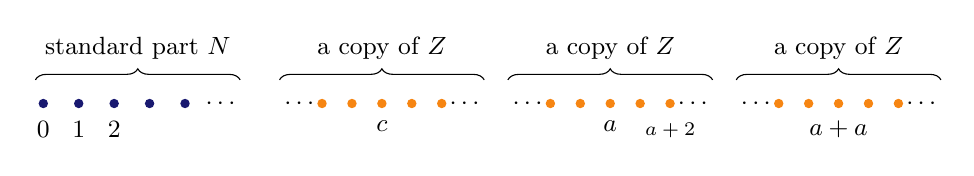
\begin{tikzpicture}[x=10mm,y=10mm,every node/.style={font=\small}]
\fill[MidnightBlue] (0.00,0) circle (1.7pt);
\fill[MidnightBlue] (0.45,0) circle (1.7pt);
\fill[MidnightBlue] (0.90,0) circle (1.7pt);
\fill[MidnightBlue] (1.35,0) circle (1.7pt);
\fill[MidnightBlue] (1.80,0) circle (1.7pt);
\node[below] at (0,-0.1) {$0$};
\node[below] at (0.45,-0.1) {$1$};
\node[below] at (0.9,-0.1) {$2$};
\node at (2.25,0) {$\cdots$};
\draw[decorate,decoration={brace,amplitude=4pt}] (-0.1,0.3) -- (2.5,0.3) node[midway,above=4pt] {standard part $\mathbb N$};
\fill[BurntOrange] (3.54,0) circle (1.7pt);
\fill[BurntOrange] (3.92,0) circle (1.7pt);
\fill[BurntOrange] (4.30,0) circle (1.7pt);
\fill[BurntOrange] (4.68,0) circle (1.7pt);
\fill[BurntOrange] (5.06,0) circle (1.7pt);
\node at (3.25,0) {$\cdots$};
\node at (5.35,0) {$\cdots$};
\node[below] at (4.30,-0.1) {$c$};
\draw[decorate,decoration={brace,amplitude=4pt}] (3.00,0.3) -- (5.60,0.3) node[midway,above=4pt] {a copy of $\mathbb Z$};
\fill[BurntOrange] (6.44,0) circle (1.7pt);
\fill[BurntOrange] (6.82,0) circle (1.7pt);
\fill[BurntOrange] (7.20,0) circle (1.7pt);
\fill[BurntOrange] (7.58,0) circle (1.7pt);
\fill[BurntOrange] (7.96,0) circle (1.7pt);
\node at (6.15,0) {$\cdots$};
\node at (8.25,0) {$\cdots$};
\node[below] at (7.20,-0.1) {$a$};
\node[below,font=\scriptsize] at (7.96,-0.12) {$a+2$};
\draw[decorate,decoration={brace,amplitude=4pt}] (5.90,0.3) -- (8.50,0.3) node[midway,above=4pt] {a copy of $\mathbb Z$};
\fill[BurntOrange] (9.34,0) circle (1.7pt);
\fill[BurntOrange] (9.72,0) circle (1.7pt);
\fill[BurntOrange] (10.10,0) circle (1.7pt);
\fill[BurntOrange] (10.48,0) circle (1.7pt);
\fill[BurntOrange] (10.86,0) circle (1.7pt);
\node at (9.05,0) {$\cdots$};
\node at (11.15,0) {$\cdots$};
\node[below] at (10.10,-0.1) {$a+a$};
\draw[decorate,decoration={brace,amplitude=4pt}] (8.80,0.3) -- (11.40,0.3) node[midway,above=4pt] {a copy of $\mathbb Z$};
\end{tikzpicture}
